\chapter{Implementación y diseño de los controles}

\section{Introducción}

El sistema de controles en Copper permite la manipulación de la escena 3D y la
interacción directa con los objetos SDF (Signed Distance Fields). Este capítulo
describe en profundidad la arquitectura, matemáticas y tecnologías utilizadas,
y se divide en dos apartados: controles de interfaz gráfica (ImGui) y controles
de gizmo (GizmoControls).

\section{Controles de interfaz gráfica: ImGui}

El módulo de interfaz gráfica (\texttt{Interfaz.cpp}, \texttt{Interfaz.h})
utiliza \textbf{ImGui} para implementar menús, sliders y herramientas de
edición.

\subsection{Estructura y funciones principales}

La clase \texttt{Interfaz} interactúa con los módulos \texttt{Coder} y
\texttt{Renderer} para:
\begin{itemize}
    \item Mostrar propiedades de objetos seleccionados (posición, color, tipo, tamaño).
    \item Permitir la edición directa mediante sliders y campos de entrada.
    \item Gestionar la creación, edición y borrado de objetos SDF.
    \item Proporcionar controles globales de la escena (luz, renderizado, operaciones).
    \item Implementar la gestión de archivos para guardar y cargar escenas.
\end{itemize}

\begin{figure}[H]
	\centering
	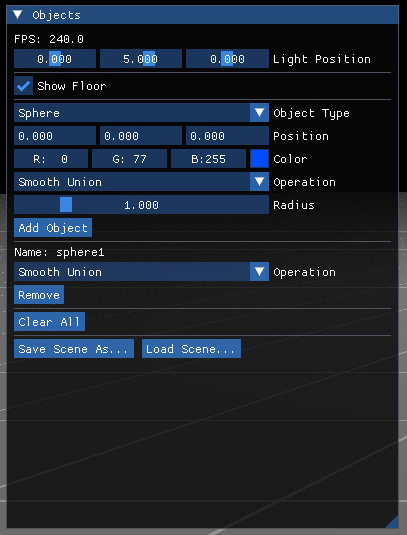
\includegraphics[width=0.7\textwidth]{imagenes/ImGui.png}
	\caption{Interfaz gráfica ImGui general.}
\end{figure}


\subsection{Ejemplo de interacción}

Al seleccionar un objeto, ImGui presenta sus propiedades y permite
modificarlas:
\begin{lstlisting}[language=C++,caption={Edición de propiedades de un objeto SDF seleccionado}]
ImGui::SliderFloat("X", &selectedObject.x, -10.0f, 10.0f);
ImGui::ColorEdit3("Color", &selectedObject.r);
// Para esferas:
ImGui::SliderFloat("Radius", &selectedObject.size[0], 0.1f, 5.0f);
\end{lstlisting}
Cada cambio marca el pipeline como "dirty" para que el renderizador actualice
la escena en tiempo real.

\begin{figure}[H]
	\centering
	\includegraphics[width=0.7\textwidth]{imagenes/ImGui_selected.png}
	\caption{Interfaz gráfica ImGui del objeto seleccionado.}
\end{figure}

\section{Controles de gizmo: GizmoControls}

El módulo \texttt{GizmoControls} (\texttt{GizmoControls.cpp},
\texttt{GizmoControls.h}) permite la manipulación visual e interactiva de los
objetos SDF seleccionados mediante gizmos (flechas, planos).

\begin{figure}[H]
	\centering
	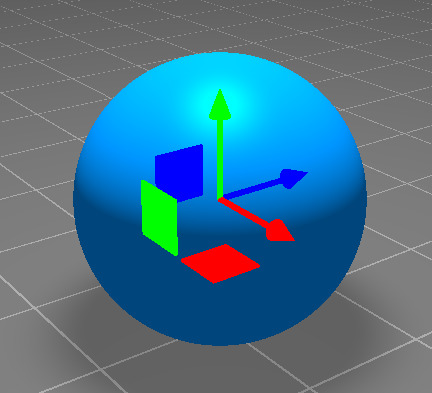
\includegraphics[width=0.7\textwidth]{imagenes/gizmo.jpg}
	\caption{Visualización de gizmo de manipulación.}
\end{figure}

\subsection{Arquitectura y flujo de interacción}

\begin{itemize}
    \item \textbf{Inicialización}: Al seleccionar un objeto y pulsar sobre el gizmo, se inicia la manipulación (\texttt{initDrag}).
    \item \textbf{Picking}: Se determina qué parte del gizmo ha sido seleccionada (eje, plano) usando ray marching y cálculos de distancia mínimos.
    \item \textbf{Arrastre y movimiento}: El punto de intersección inicial se calcula con \texttt{gizmoIntersection} y se actualiza en tiempo real mientras el usuario mueve el ratón.
    \item \textbf{Actualización de propiedades}: El centro del objeto se actualiza en \texttt{update}, propagando el nuevo valor al objeto seleccionado en el módulo \texttt{Coder}.
\end{itemize}


\subsection{Gizmo de movimiento lineal en ejes X, Y y Z}

Para implementar el gizmo de movimiento lineal, es necesario implementar un
sistema que detecte la cantidad de movimiento en cada eje con respecto al
desplazamiento del ratón. Esto significa transformar unas coordenadas
\textit{screen space} (2D) a coordenadas \textit{world space} (3D).

El sistema implementado se basa en la intersección entre dos líneas en
\text{world space}, una línea que representa al eje sobre el que queremos mover
el objeto, y otra línea, que representa el rayo \textit{casteado} desde la
posición del ratón. Este último rayo parte de la posición de la cámara y se
extiende hacia el plano de la escena. La sección de \textit{raymarching}
explica como transformar una coordenada UV de la pantalla a rayos casteados
desde la posición de la cámara.

Como en 3D es difícil hacer que dos líneas se crucen, y la precisión perdida en
las aproximaciones de coma flotante podría afectar a los cálculos. Hemos
decidido utilizar una expresión para el punto más cercano entre dos líneas.
Estas expresiones son ampliamente conocidas y se puede encontrar en múltiples
fuentes. A continuación se deja un desarrollo propio.

Sean dos líneas en el espacio 3D, definidas por sus ecuaciones paramétricas:

\begin{equation}
    \begin{cases}
        p_1 = k_1 + l_1  \vec{v}_1, \\
        p_2 = k_2 + l_2  \vec{v}_2.
    \end{cases}
\end{equation}

Dónde $k_1$ y $k_2$ son dos puntos por los que pasan las líneas, $\vec{v}_1$ y
$\vec{v}_2$ son sus vectores directores, y $l_1$ y $l_2$ son los parámetros que
recorren las líneas, dos números reales. La distancia entre dos puntos
arbitrarios en cada línea, $p_1$ y $p_2$, se puede expresar como:

\begin{equation}
    d = \| p_1 - p_2 \| = \| (k_1 + l_1 * \vec{v}_1) - (k_2 + l_2 * \vec{v}_2) \|.
\end{equation}

Descomponiendo los vectores y puntos en sus componentes y tomando el cuadrado
de la distancia, obtenemos:

\begin{equation}
    \begin{align}
        d^2 = & \left(k_{1_x} + l_1 v_{1_x} - k_{2_x} - l_2 v_{2_x}\right)^2  \\
        +     & \left(k_{1_y} + l_1 v_{1_y} - k_{2_y} - l_2 v_{2_y}\right)^2  \\
        +     & \left(k_{1_z} + l_1 v_{1_z} - k_{2_z} - l_2 v_{2_z}\right)^2.
    \end{align}
\end{equation}

Teniendo en cuenta que solo tenemos dos variables, ambas al cuadrado, podemos
ver que \(d^2\) es una parábola tridimensional. Como la parábola es positiva,
todos los puntos están por encima de $d = 0$, solo tiene un mínimo, el mínimo
global. Nuestro problema tiene por tanto una sola solución, que podemos
encontrar buscando este mínimo, (no tendremos que descartar puntos de silla).

El mínimo lo encontraremos en el punto en el que la derivada de $d^2$ con
respecto a $l_1$ y $l_2$ sea cero.

\begin{align}
     & \begin{align}
           \frac{\partial d^2}{\partial l_1} = 0 = 2\left(k_{1_x} + l_1 v_{1_x} - k_{2_x} - l_2 v_{2_x}\right)v_{1_x} \\
           + 2\left(k_{1_y} + l_1 v_{1_y} - k_{2_y} - l_2 v_{2_y}\right)v_{1_y}                                       \\
           + 2\left(k_{1_z} + l_1 v_{1_z} - k_{2_z} - l_2 v_{2_z}\right)v_{1_z},
       \end{align}  \\
     & \begin{align}
           \frac{\partial d^2}{\partial l_2} = 0 = -2\left(k_{1_x} + l_1 v_{1_x} - k_{2_x} - l_2 v_{2_x}\right)v_{2_x} \\
           -2\left(k_{1_y} + l_1 v_{1_y} - k_{2_y} - l_2 v_{2_y}\right)v_{2_y}                                         \\
           + 2\left(k_{1_z} + l_1 v_{1_z} - k_{2_z} - l_2 v_{2_z}\right)v_{2_z}.
       \end{align}
\end{align}
Desarrollando estas ecuaciones podemos obtener:

\begin{align}
    l1 & = \frac{l_2 \vec{v}_2\cdot\vec{v}_2 - k_1\cdot k_2 + k_2\cdot k_2 } { v_1\cdot v_2},                                                                                                                                                                               \\
    l2 & = \frac{\frac{\vec{v}_1\cdot{\vec{v}_1}}{\vec{v}_1\cdot\vec{v}_2}(k_2\cdot\vec{v}_2 - k_1\cdot\vec{v}_2) + k_1\cdot \vec{v}_1 - k_2\cdot\vec{v}_1}{\vec{v}_1\cdot\vec{v}_2 - \frac{(\vec{v}_2\cdot\vec{v}_2) (\vec{v}_1\cdot\vec{v}_1)}{\vec{v}_1\cdot\vec{v}_2}},
\end{align}
los parámetros que debemos introducir en las ecuaciones paramétricas de las líneas para obtener los puntos más cercanos entre ambas.

\subsection{Gizmo de movimiento en planos XY, XZ y YZ}

El movimiento en un plano del gizmo (por ejemplo, el plano XY) utiliza un
enfoque geométrico distinto al del movimiento lineal. En lugar de encontrar la
distancia mínima entre dos líneas, el sistema calcula la intersección directa
entre el rayo del ratón y el plano de movimiento.

El proceso, implementado en las funciones \texttt{GizmoControls::update} y
\texttt{gizmoIntersection}, es el siguiente:

\begin{enumerate}
    \item \textbf{Definición del plano}: Cuando se selecciona un gizmo de plano (por ejemplo, el plano XY), el sistema lo define mediante un punto que contiene (el centro del objeto, \texttt{objectCenter}) y su vector normal. Es importante destacar que, por convención en el código, el vector almacenado en \texttt{currentGizmo} para un plano es su normal. Por ejemplo, para el plano XY, la normal es el eje Z (0, 0, 1).
    \item \textbf{Intersección Rayo-Plano}: Con cada movimiento del ratón, se vuelve a castear un rayo desde la cámara (\texttt{ro}, \texttt{rd}). La función \texttt{planeLineIntersection} calcula el punto exacto donde este rayo intersecta el plano infinito definido en el paso anterior. La ecuación para la intersección de una línea y un plano es una fórmula geométrica estándar.
    \item \textbf{Cálculo del Desplazamiento}: El sistema calcula el vector de desplazamiento (\texttt{diffV}) restando el punto de intersección inicial (\texttt{firstIntersectionPoint}, calculado en \texttt{initDrag}) del punto de intersección actual.
          \begin{verbatim}
glm::vec3 diffV = intersection - this->firstIntersectionPoint;
    \end{verbatim}
    \item \textbf{Aplicación del Movimiento Restringido}: El desplazamiento \texttt{diffV} se suma a la posición inicial del objeto (\texttt{initialObjectCenter}) para obtener la nueva posición teórica. Sin embargo, para asegurar que el objeto solo se mueva en el plano seleccionado, se aplica una máscara vectorial. Esta máscara se crea restando el vector normal del plano al vector identidad \texttt{glm::vec3(1.0)}.
          \begin{itemize}
              \item Para el plano XY, la normal es (0, 0, 1). La máscara es (1, 1, 1) - (0, 0, 1) =
                    (1, 1, 0).
              \item Para el plano XZ, la normal es (0, 1, 0). La máscara es (1, 1, 1) - (0, 1, 0) =
                    (1, 0, 1).
              \item Para el plano YZ, la normal es (1, 0, 0). La máscara es (1, 1, 1) - (1, 0, 0) =
                    (0, 1, 1).
          \end{itemize}
          Al multiplicar la nueva posición por esta máscara, se anula cualquier movimiento en la dirección de la normal, restringiendo el desplazamiento exclusivamente al plano deseado.
\end{enumerate}

Este método garantiza que, aunque el ratón se mueva en un espacio 2D y el rayo
viaje en 3D, el objeto seleccionado se deslice perfectamente sobre el plano
elegido, proporcionando un control intuitivo y preciso.